\documentclass[beamer]{standalone}
\usepackage{../templates/common}
\usepackage{../templates/phylofig}

\begin{document}
\begin{standaloneframe}
\centering
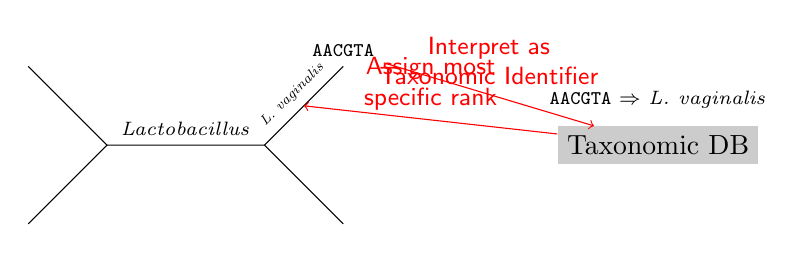
\begin{tikzpicture}
    \draw (0,1) -- (1,0) -- (0,-1);
    \draw (1,0) -- (3, 0) -- (4,-1);
    \draw (3,0) -- (4,1);
    \node[above] at (2,0) {\scriptsize \textit{Lactobacillus}};
    
    \node[above] (seq) at (4,1) {\scriptsize\texttt{AACGTA}};
    \node[rectangle, fill=black!20] (db) at (8,0) {Taxonomic DB};
    \onslide<1-2>{\path[every node/.style={font=\sffamily\small}, ->, red]
    (seq) edge node [right, above, align=center] {Interpret as\\ Taxonomic Identifier} (db);}
    
    \onslide<2->{\node[above] at (8,.35) {\scriptsize{\texttt{AACGTA}} $\Rightarrow$ \textit{L. vaginalis}};}
    
    \onslide<3->{\path[every node/.style={font=\sffamily\small}, ->, red]
    (db) edge node [right, above, align=center] {Assign most\\ specific rank} (3.5,0.5);}

    \node<4>[above, rotate=45] at (3.5,0.5) {\tiny \textit{L. vaginalis}};
\end{tikzpicture}
\end{standaloneframe}
\end{document}
